% -*- root: ../AlgebraConmutativa.tex -*-
\chapter{Anillos II}

\section{Módulos sobre anillos}
Sea $R$ un anillo, diremos que $M$ es un \concept{{$R$}-módulo} o módulo sobre $R$ si se cumplen las siguientes condiciones:
\begin{enumerate}
	\item $(M,+)$ es un grupo abeliano.
	\item Hay una operación externa sobre $M$.
		\begin{align*}
			R×M & \longmapsto  M \\
			(r,m) & \longmapsto  r\cdot m \\
		\end{align*}

	tal que se cumplen las siguientes propiedades, a las que llamaremos \textbf{propiedades romanas} o \textbf{propiedades sensatas}:
	\begin{itemize}
		\item $\forall r \in R, \forall m,m' \in M$: $r(m+m')=rm+rm'$.
		\item $\forall r,r' \in R, \forall m \in M$: $(r+r')m=rm+r'm$.
		\item $\forall r,r' \in R, \forall m \in M$: $r(r'm)=(rr')m$.
		\item $\forall m \in M$, $\one_R\cdot m = m$.
	\end{itemize}
\end{enumerate}

\begin{example}
	\begin{itemize}
		\item Si $R$ es un cuerpo $\implies$ cualquier espacio vectorial sobre $R$ es un módulo sobre $R$.
		\item Si $I \subset R$ es un ideal $\implies$ $I$ es un $R$-módulo. Por tanto, en particular $R$ es un $R$-módulo.
		\item Sea $f: R \longmapsto S$ un homomorfismo de anillos, sea $J \subset S$ un ideal $\implies$ $J$ es un $R$-módulo.
		\begin{proof}
			De esté último ejemplo, tenemos que ver que se cumplen las propiedades de los $R$-módulos:
			\begin{enumerate}
				\item $(J,+)$ es un subgrupo por ser ideal.
				\item Definimos la operación externa:
				\begin{align*}
					R×J & \longmapsto  J \\
					(r,a) & \longmapsto  f(r)\cdot a \\
				\end{align*}

				Defino $r\cdot a=f(r)\cdot a$. Ahora tenemos que ver que se cumplen las propiedades sensatas, demostramos la primera y las demás las dejamos como ejercicio para el lector con mucho tiempo libre:
				\begin{itemize}
					\item $\forall r \in R, \forall a,a' \in J$, $r(a+a')=ra+ra'$:

					Por definición de la operación externa tenemos que: $r(a+a')=f(r)(a+a')$. Por la propiedad distributiva de $S$ tenemos que $f(r)(a+a')=f(r)a+f(r)a'$. Aplicando de nuevo la definición de producto externo $f(r)a+f(r)a'=ra+ra'$.
				\end{itemize}
			\end{enumerate}
		\end{proof}
	\end{itemize}
\end{example}

Más ejemplos:
\begin{example}
	\begin{itemize}
		\item El ideal $\gen{x}$ en $\ent[x]$ es un $\ent$-módulo.
		\item Sea $I \subset R$ un ideal, sea $\pi:R\longmapsto \quot{R}{I}$ un homomorfismo de anillos, todo ideal de $\quot{R}{I}$ es un $R$-módulo.
		\item Sea $f:R \longmapsto S$ un homomorfismo de anillos. Entonces S es también un $R$-módulo.
		\item Todo anillo $R$ es un $\ent$-módulo. Para ello basta comprobar que siempre hay un homomorfismo de anillos de $\ent$ en R.
		\begin{align*}
			g:\ent &\longmapsto  R\\
			1 & \longmapsto \one_R \\
			m & \longmapsto  m\cdot \one_R \\
		\end{align*}

		Con esto defino el homomorfismo porque 1 genera $\ent$ como grupo.

		Es más, todo anillo $R$ contiene una copia de $\ent$ o una copia de algún $\ent_n$. Basta observar que $\ent/\ker(g) \simeq \img(g) \subset R$. Por tanto hay dos casos:
		\begin{enumerate}
			\item Si $\ker(g)=(0) \implies \ent \simeq \img(g) \subset R$
			\item Si $\ker(g)=\gen{n}\implies \ent_n \simeq \img(g) \subset R$ para $n\in \ent$ con $n\neq0$ y $n\neq 1,-1$ (porque $1\notin \ker(g)$).
		\end{enumerate}
	\item En $\ent_{10}$ cogemos $M=\gen{2}=\{\cls{0},\cls{2},\cls{4},\cls{6},\cls{8} \}$

	M es también un $\ent_5$-módulo (aparte de un $\ent_{10}$-módulo y un $\ent$-módulo), ya que:
	\begin{enumerate}
		\item $(M,+)$ es un grupo abeliano, al ser ideal.
		\item Definimos la operación externa:
		\begin{align*}
			\ent_5 × M & \longmapsto  M \\
			(\cls{a},\cls{m}) & \longmapsto  \cls{a}\cdot \cls{m} =\cls{a\cdot m} \\
		\end{align*}

		Vamos a ver que este producto está bien definido, es decir, que no depende de los representantes escogidos: $\cls{a}=a+5l$, y $\cls{m}=2n+10k$. Operamos:
		$$\cls{a}\cdot \cls{m}=a2n+10ak+10lm+50lk \underbrace{\equiv}_{mod 10} a2n=\cls{a2n}=\cls{a}\cls{2n}$$

		Vemos que efectivamente esta operación no depende de los representantes obtenidos y por tanto está bien definida. faltaría comprobar las propiedades romanas (o sensatas) y ya está (pero not today).
		\item Sin embargo en el ejemplo anterior $M$ no es un $\ent_3$-módulo. Por ejemplo, en $\ent_3$ es lo mismo 1 que 4. Sin embargo, cogiendo $\cls{2}\in M$, no es lo mismo $4\cdot\cls{2}=8=\cls{8}$ que $1\cdot\cls{2}=2=\cls{2}$.
	\end{enumerate}
	\end{itemize}
\end{example}

\begin{defn}[R-módulo\IS finitamente generado]\label{def:rmodulo_fg}
	Sea $M$ un $R$-módulo, diremos que $M$ es un $R$-módulo finitamente generado si $\exists m_1,\dots,m_s \in M$ tal que $M=\{r_1m_1+\dots+r_sm_s: r_i \in R \}$.

	Es decir $\exists m_1..., m_n \in M$ tales que cada elemento de M es una combinación lineal de esos elementos con coeficientes del anillo escalar R.
\end{defn}

\begin{example}
	\begin{itemize}
	\item Sea $\ent$, cogemos $I=\gen{a}$ con $a\in \ent$. I es un $\ent$-módulo finitamente generado ya que $I=\{na:n \in \ent \}$. Cada elemento de $M$ se puede escribir como $a$ multiplicado por algún elemento de $\ent$.
	\item Sea $K[x]$, cogemos $I \subset K[x]$ con $I=\gen{p(x)}=\{ q(x)p(x): q(x) \in K[x] \}$. $I$ es un $K[x]$-módulo finitamente generado.
	\item Sea $\rac[x,y]$ cogemos $I=\{ p(x,y):p(0,0)=0 \}=\gen{x,y}=\{ xp(x,y)+yr(x,y): p,q \in \rac[x,y] \}$. $I$ es un $\rac[x,y]$-módulo finitamente generado.
	\item $\ent[x]$ no es un $\ent$-módulo finitamente generado.

	\begin{proof}
		Supongamos que $\ent[x]$ fuera finitamente generado como $\ent$-módulo. Entonces $\exists p_1(x),\dots,p_r(x) \in \ent[x]$ tales que $\ent[x]\{ n_1p_1(x)+\dots+n_rp_r(x): n_i \in \ent \}$. Sea $m=\max\{grado(p_i(x)) \} \implies grado(n_1p_1(x)+\dots+n_rp_r(x)) \leq m$. Pero en $\ent[x]$ no hay grado máximo.

		Sin embargo $\ent[x]$ si es una $\ent$-álgebra finitamente generada, o una $\ent$-algebra de tipo finito ya que:
		$$ \ent[x]=\set{ \sum_{i=0}^n a_i x^i: a_i \in \ent, n \in \nat }$$
	\end{proof}
	\item Sea $\rac \subset \rac[\sqrt{2}]$.

	Es un $\rac$-módulo finitamente generado ya que $\rac[\sqrt{2}]=\{ a+b\sqrt{2}:a,b \in \rac \}$.

	Es también una $\rac$-algebra ya que $\rac[\sqrt{2}]=\{ \sum_{i=0}^n a_i(\sqrt{2})^i :a_i \in \rac, n \in \nat \}$
\end{itemize}
\end{example}

\begin{defn}[R-álgebra\IS finitamente generada]\label{def:ralgebra_fg}
	Sea $f: R \longmapsto S$ un homomorfismo de anillos. Entonces $S$ es una $R$-álgebra vía f (ver \ref{def:ralgebra}). Diremos que S es una $R$-álgebra finitamente generada (o de tipo finito) si $\exists \alpha_1,\dots, \alpha_s \in S$ tal que:
	$$ S=\left\{ \sum_{finito} f(a_{i1}\dots a_{ir})\alpha_1^{i1}\dots\alpha_r^{ir}: a_{i1},\dots, a_{ir} \in R \right\} $$
\end{defn}

\begin{example}
	\begin{itemize}
		\item Sea $\real \longmapsto \real[x]$. Tomamos $\alpha_1=x$, y entonces $\real[x]=\left\{ \sum_{i=1}^n a_ix^i: a_i \in \real, n\in \nat  \right\}$
		\item Sea $R \longmapsto R[x_1,\dots,x_n]$ no es un $R$-módulo finitamente generado pero si es una $R$-álgebra de tipo finito, porque podemos coger $\alpha_1=x_1,\dots,\alpha_n=x_n$.
		\item Sea $R \longmapsto R[x_1,...,x_n,...]$ (número infinito de variables) entonces no es ni $R$-módulo ni $R$-álgebra.
		\item Sea $\rac \longmapsto \rac[\sqrt{2}]$ es una $\rac$-álgebra finitamente generada (la genera $\sqrt{2}$) y un $\rac$-módulo finitamente generado (lo genera $\{ 1, \sqrt{2} \}$).
		\item Sea $\real$, es una $\rac$-álgebra pero no es de tipo finito (si lo fuera $\real$ sería numerable). Es un $\rac$-módulo.
	\end{itemize}
\end{example}

\begin{defn}[R-submódulo]
	Sea $M$ un $R$-módulo. Diremos que $N \subset M$ es un $R$-submódulo de $M$ si $N$ es un $R$-módulo.
\end{defn}
\begin{prop}
	Sea $M$ un $R$-módulo y sea $N \subset M$. Entonces $N$ es un $R$-submódulo $\Leftrightarrow$:
	\begin{enumerate}
		\item $N \neq \emptyset$.
		\item Si $n,m \in \nat$, $n-m \in \nat$ (lo que es equivalente a que Si $n,m \in \nat$, $n+m \in \nat$).
		\item $\forall r \in R, \forall n \in N$, $rn \in N$.
	\end{enumerate}
\end{prop}

\begin{defn}[Homomorfismo\IS de R-módulos]
	Sean $M,L$ dos $R$-módulos y sea $f:M\longmapsto L$. Diremos que f es un homomorfismo de $R$-módulos si:
	\begin{enumerate}
		\item $\forall n,m \in M$ se tiene que $f(n+m)=f(n)+f(m)$.
		\item $\forall r \in R,\forall m \in M$, se tiene que $f(rm)=rf(m)$.
	\end{enumerate}
\end{defn}

\begin{defn}[Homomorfismo\IS de R-álgebras]
	Sea $R\subset A,B$ tenemos un homomorfismo $f: A \rightarrow B$, $f$ es homomorfismo de $R$-álgebras si todos los elementos de $R$ van a parar a sí mismos.
\end{defn}

\begin{example}
	Cogemos $R= \ent$, $M=\gen{2}$ y $N=\gen{3}$. El homomorfismo sería:
	\begin{align*}
		f: \gen{2} & \longmapsto  \gen{3}\\
		x & \longmapsto 3x \\
	\end{align*}


	\obs De $\ent \longmapsto \ent$ no se puede hacer ya que $x \longmapsto 3x$ mandaría el \one al 3 y el \one tiene que ir al \one.
\end{example}

\begin{defn}[Núcleo\IS de homomorfismo de R-modulos]
	Sea $f:M \longmapsto N$ un homomorfismo de $R$-módulos. Definimos $\ker(f)=\{ m\in M:f(m)=0 \}$.
\end{defn}

\obs $\ker(f)$ es un submódulo de M. (Si no te lo crees, lo demuestras).

\begin{defn}[Cociente\IS de módulos]
Si $N \subset M$ es un submódulo de M, se define de manera natural el cociente $\quot{N}{M}$, $m,m' \in M$, $m~m'$ si $m-m' \in N$. Y $\quot{M}{N}$ es un $R$-modulo.
\end{defn}

Se deja como ejercicio escribir las versiones del primer y segundo teoremas de isomorfía para módulos.

\section{Tercer Teorema de isomorfía}
\begin{theorem}[Tercer teorema de isomorfía][Teorema\IS 3º de isomorfía] \label{thm:IsomorfiaAnillos3}
	Sean $I$, $J$ ideales en $R$:
	$$ \quot{I+J}{I} \simeq \quot{J}{I \cap J} $$
\end{theorem}
\begin{proof}
	Recordemos que $I+J$ es el ideal más pequeño que contiene a $I$ y a $J$.


	Sea $\pi: R \longmapsto \quot{R}{I}$, sabemos que $\pi$ es sobreyectiva y que $\ker(\pi)=I$. Por tanto, $\pi(I)=0$, y $\pi(I+J)=\pi(J)$ es un ideal.

	Además, pues que $\pi$ no es más que una aplicación de paso al cociente, tenemos que $\pi(J)=\pi(J+I)=\quot{J+I}{I}$. Definimos la siguiente función sobreyectiva:

	$$ \cls{\pi}=\pi|_J: J \longmapsto \quot{J+I}{I}  $$

	Por el primer teorema de isomorfía, se tiene que:
	$$ \quot{J}{\ker(\cls{\pi})} \simeq \quot{J+I}{I} $$

	Entonces vamos a calcular $\ker(\cls{\pi})$. Que serán los elementos de $I$. Pero como no necesariamente esta $I\subset J$, entonces cogemos los elementos de $I$ que también pertenecen a $J$. Es decir $\ker(\cls{\pi})=I \cap J$, por tanto:

	$$ \quot{J}{I \cap J} \simeq \quot{J+I}{I} $$

\end{proof}


\begin{example}
	Cogemos $\gen{4}$ y $\gen{6}$ contenidos en $\ent$. Por el tercer teorema de isomorfía tenemos:
	$$ \quot{\gen{4}+\gen{6}}{\gen{4}}\simeq \quot{\gen{6}}{\gen{6} \cap \gen{4}} $$

	Lo comprobamos:
	$$\quot{\gen{4}+\gen{6}}{\gen{4}} = \quot{\gen{2}}{\gen{4}}=\{ \cls{0} \cls{2} \}$$

	$$ \quot{\gen{6}}{\gen{6} \cap \gen{4}} = \quot{\gen{6}}{\gen{12}} = \{ \cls{0}, \cls{6} \}$$

	El isomorfismo sería:
	\begin{align*}
		\cls{0}  & \longmapsto  \cls{0}\\
		\cls{6} & \longmapsto \cls{2} \\
	\end{align*}
\end{example}

\section{Localización en una parte multiplicativa}
\begin{defn}[Parte\IS multiplicativa]
	Sea $R$ un anillo y sea $S\subset R$ un subconjunto. Diremos que $S$ es una parte multiplicativa en $R$ o un conjunto multiplicativamente cerrado en $R$ si se cumplen las siguientes condiciones:
	\begin{enumerate}
		\item $\one \in S$
		\item $s,s' \in S \implies s\cdot s' \in S$.
	\end{enumerate}
\end{defn}

Por tanto, intuitivamente vemos que

\begin{example}
	\begin{itemize}
		\item Sea $R$, cogemos $S=\{\one \}$
		\item Sea $R$, cogemos $S=U(R)$ (Unidades de R).
		\item Sea $a \in R$, cogemos $S=\{ a^n: n \in \nat \}$.
		\item Sea $p \subset R$ un ideal primo. Cogemos $S=R \setminus p$. Este ejemplo vamos a probarlo, S es una parte multiplicativa porque:
		\begin{enumerate}
			\item $\one \in S$, ya que $\one \notin p$.
			\item $s,s' \in S \implies s\cdot s' \in S$. Si ya que: $s,s' \in S \implies s,s' \notin p \implies s\cdot s' \notin p \implies s\cdot s' \in S$.
		\end{enumerate}
		\item Sea R, cogemos $S= R \setminus \{\{ \text{divisores de 0}\}\cup \{ \zero \} \}$ también es parte multiplicativa.
		\item Sea $R$, y sea $\{p_i\}_{i\in I}$ colección de ideales primos en $R$. Entonces $S=R\setminus \bigcup_{i\in I}p_i$ es una parte multiplicativa.
	\end{itemize}
\end{example}

\subsection{Construcción del localizado de R en una parte multiplicativa S}

Sea $S \subset R$. Construimos $R×S=\{ (r,s): r \in R, s\in S \}$. Podemos pensar en lugar del par $(r,s)$ en la fracción $\frac{r}{s}=s^{-1}r$, de ahí viene la expresión $S^{-1}R$. Necesitaremos además una forma de identificar elementos igual que identificamos fracciones, así que una primera relación de equivalencia en $R×S$ podría ser la siguiente: \( (r,s)\sim(r',s') \iff rs'-r's =0 \label{eq:RelEquivLocalizado_Mala} \)

Podemos definir la operación suma como, dados $(r,s), (r',s')\in R×S$, entonces $(r,s)+(r',s')=(rs',ss')+(r's,s's)=(rs'+r's,ss')$. La operación producto sería la obvia: $(r,s)+(r',s')=(rr',ss')$.

Ahora bien, lo malo de la relación de equivalencia que hemos dado en \eqref{eq:RelEquivLocalizado_Mala} es que nos puede dar problemas. Vamos a tomar $\ent_6$ y $S=\set{ \cls{1},\cls{2},\cls{4}}$ una parte multiplicativa, para construir el localizado $\inv{S}ℤ_6$.

En ese localizado podemos coger $(\cls{3},\cls{1})$ y $(\cls{0},\cls{1})$. Obviamente no están relacionados, ya que $\cls{3}\cdot\cls{1}\neq \cls{1}\cdot\cls{0}$. Podemos hacer una manipulación extra, que es multiplicar por $\cls{2}$ el primer elemento, $(\cls{3}, \cls{1})$. Esto no debería cambiar la relación de equivalencia (sólo hay que mirar la definición de \eqref{eq:RelEquivLocalizado_Mala} para verlo), pero si calculamos, tenemos que $\cls{2} · (\cls{3}, \cls{1}) = (\cls{0}, \cls{2})$ y ahora ambos elementos sí están relacionados: $\cls{0} · \cls{1} = \cls{0} · \cls{2}$. En otras palabras, algo ha fallado en la definición de relación de equivalencia y tenemos que mejorarla.

Esa mejora será definirla de la siguiente forma: \( (r,s) \sim (r', s') \iff ∃s'' ∈ S \tq s''(rs'-r's) = 0 \label{eq:RelEquivLocalizado} \)

Ahora sí podremos probar que es una relación de equivalencia:

\begin{itemize}
\item \textbf{Reflexión}: Es claro que $(r,s) \sim (r,s)$, tomando $s'' = \one ∈ S$.
\item \textbf{Simetría}: Si $(r,s) \sim (r',s')$, entonces $∃s'' ∈ S$ tal que $s'' (rs' - r's) = 0$. Declaramos que $s''$ nos vale para decir que $(r',s') \sim (r,s)$. Sea $a = s''(r's-rs')$. Podemos sumar entonces a esta ecuación la que ya sabemos que se cumple: $s''(rs'-r's) = 0$ y entonces
\begin{align*}
s''(rs'-r's) + s''(r's-rs') &= 0 + a \\
s''(rs'-r's + r's-rs') &= a \\
0 &= a
\end{align*}, por lo que efectivamente $(r',s') \sim (r,s)$.
\item \textbf{Transitividad}: No se me ocurre como probarla ahora mismo.
\end{itemize}

Así, Definimos el siguiente anillo:
 $$S^{-1}R = \left( \quot{R×S}{\sim},+,\cdot \right)$$

En el que encontramos:
\begin{itemize}
	\item Elemento neutro para $+$, que es el $(0,s)$, $\forall s \in S$ (todos ellos conforman la misma clase de equivalencia, así que no se viola la unicidad).
	\item Identidad para $\cdot$, que es $(1,1)$.
	\item Sea $(s,1) \in S^{-1}R$, su inverso es $(1,s) \in S^{-1}R$.
\end{itemize}

Vamos a ver $R$ en $S^{-1}R$. Para ello construimos una función de $R$ en $S^{-1}R$ de la siguiente manera:
\begin{align*}
	R & \longmapsto  S^{-1}R\\
	r & \longmapsto (r,1) \\
\end{align*}

Esta aplicación es un homomorfismo de anillos, y podremos estudiar propiedades de los elementos de $\inv{S}R$ a través de él.

Por ejemplo, podemos estudiar su núcleo, que serán los elementos cuya imagen sea la clase de $0_{\inv{S} R}$, que es de la forma $(0,s)$. Simplemente aplicando $f$, tenemos que tener $(r, 1) \sim (0,s)$, lo que nos lleva a la definición verdaderamente útil del núcleo: \[ \ker f = \set{r ∈ R \tq ∃s ∈ S,\, s'r = 0_R} \]

Este homomorfismo no siempre es inyectivo.

\begin{prop}
	$S^{-1}R=\{ 0 \} \Leftrightarrow 0 \in S \Leftrightarrow S$ contiene nilpotentes.
\end{prop}

\begin{prop}
	Si $S^{-1}R \neq \{ 0 \} \implies f(s)$ es invertible en $S^{-1}R\; \forall s \in S$
\end{prop}

\begin{example} \textbf{Importante para practicar con parte multiplicativa y repasar lo anterior}
	Sea $R = \ent_6$ y $S=\{ \cls{1}, \cls{2}, \cls{4} \}$

	Vamos a estudiar $S^{-1}\ent_6$, para ello seguimos los siguientes pasos:

	Definimos el homomorfismo tal y como hemos dicho:
	\begin{align*}
		f: \ent_6 & \longmapsto  S^{-1}\ent_6\\
		\cls{0} & \longmapsto (\cls{0},\cls{1}) \\
		\cls{n} & \longmapsto (\cls{n},\cls{1}) \\
	\end{align*}

Calculamos el núcleo: $\ker(f)=\{ r \in R: \exists s' \in S: s'r=0 \}$. Es decir
$$\ker(f) = \{ r \in \ent_6: \exists s' \in \{ \cls{1}, \cls{2}, \cls{4} \}: s'r=0_{\ent_6} \} = \{ \cls{0}, \cls{3}\}$$

\textcolor{blue}{Demostracion a saco (cuentas tontas):
	\begin{itemize}
		\item $\cls{0} \in \ker(f)$ ya que $s'\cls{0}=\cls{0}$, $\forall s' \in S$
		\item $\cls{1} \notin \ker(f)$ ya que $s'\cls{1}\neq\cls{0}$, $\forall s' \in S$: $\cls{1}\cdot\cls{1}=\cls{1}$, $\cls{2}\cdot\cls{1}=\cls{2}$ y $\cls{4}\cdot\cls{1}=\cls{4}$
		\item $\cls{2} \notin \ker(f)$ ya que $s'\cls{2}\neq\cls{0}$, $\forall s' \in S$: $\cls{1}\cdot\cls{2}=\cls{2}$, $\cls{2}\cdot\cls{2}=\cls{4}$ y $\cls{4}\cdot\cls{2}=\cls{2}$
		\item $\cls{3} \in \ker(f)$ ya que $s'\cls{3}=\cls{0}$ cogiendo $s'=\cls{2}$ o $s'=\cls{4}$
		\item $\cls{4} \notin \ker(f)$ ya que $s'\cls{4}\neq\cls{0}$, $\forall s' \in S$: $\cls{1}\cdot\cls{4}=\cls{4}$, $\cls{2}\cdot\cls{4}=\cls{2}$ y $\cls{4}\cdot\cls{4}=\cls{4}$
		\item $\cls{5} \notin \ker(f)$ ya que $s'\cls{5}\neq\cls{0}$, $\forall s' \in S$: $\cls{1}\cdot\cls{5}=\cls{5}$, $\cls{2}\cdot\cls{5}=\cls{4}$ y $\cls{4}\cdot\cls{5}=\cls{2}$
	\end{itemize}}

	Ahora vamos a usar el primer teorema de isomorfía. Por el cual sabemos que existe un homomorfismo de anillos:
	$$\cls{f}: \quot{\ent_6}{\gen{\cls{3}}} \longmapsto S^{-1}\ent_6$$

	\textbf{Notacion:}
	\begin{itemize}
		\item $\ent_6 = \quot{\ent}{\gen{6}}= \quot{\ent}{6 \ent}$.
		\item En este caso $\gen{\cls{3}}$ es el ideal generado por $\cls{3}$ dentro del ideal $6\ent=\gen{6}$ en $\ent$. Es decir, que en este caso se cumple: $\gen{\cls{3}}=\quot{3\ent}{6\ent} = \{ \cls{0}, \cls{3}\}$ como hemos visto.
	\end{itemize}

	Ahora aplicamos el segundo teorema de isomorfía. Para ello necesitamos $I \subset J \subset R_1$. Cogemos $R_1 = \ent$, $J=\gen{3}$ e $I=\gen{6}$. Por el segundo teorema de isomorfía:

	$$ \quot{\ent_6}{\gen{\cls{3}}} \simeq \quot{\quot{\ent}{\gen{6}}}{\quot{\gen{3}}{\gen{6}}} \underbrace{\simeq}_{2º \text{tma isomorfía} } \quot{\ent_6}{\gen{3}} \simeq \ent_3$$

	Ahora volvemos a aplicar el primer teorema de isomorfía, pero la segunda parte, la que nos dice que: $\quot{R}{\ker(f)} \simeq \img(f)$. En nuestro caso tenemos $R=\ent_6$, y $\ker(f)=\gen{\cls{3}}$, y como acabamos de ver  $\quot{\ent_6}{\gen{\cls{3}}}$ es isomorfo $\ent_3$. Por tanto no queda otra que:

	$$\img(f) \simeq \ent_3$$

	Sabiendo podemos definir $f$ de forma mucho más precisa:
	\begin{align*}
		f: \ent_6 & \longmapsto  S^{-1}\ent_6 \simeq \ent_3\\
		\cls{0} & \longmapsto (\cls{0},\cls{1}) \\
		\cls{1} & \longmapsto (\cls{1},\cls{1}) \\
		\cls{2} & \longmapsto (\cls{2},\cls{1}) \\
		\cls{3} & \longmapsto (\cls{0},\cls{1}) \\
		\cls{4} & \longmapsto (\cls{1},\cls{1}) \\
		\cls{5} & \longmapsto (\cls{2},\cls{1}) \\
	\end{align*}

	Ahora podemos ver las equivalencias entre los elementos de $S^{-1}\ent_6$, algunos ejemplos son:
	\begin{itemize}
		\item $(\cls{1},\cls{4})\equiv (\cls{1},\cls{1})$ porque $\cls{1}\cdot \cls{4} = \cls{4} = \cls{1} =\cls{1}\cdot \cls{1}$.
		\item $(\cls{2},\cls{1}) \equiv (\cls{1},\cls{2})$ ya que $\cls{2}\cdot \cls{2} = \cls{4} = \cls{1} =\cls{1}\cdot \cls{1}$.
		\item $(\cls{4},\cls{1}) \equiv (\cls{2},\cls{2})$ ya que $\cls{4}\cdot \cls{2} = \cls{8} = \cls{2} =\cls{1}\cdot \cls{2}$.
		\item $(\cls{2}, \cls{2}) = (\cls{2},\cls{1}) \cdot (\cls{1},\cls{2}) \equiv (\cls{4},\cls{1}) $.
		\item $(\cls{2},\cls{1}) \cdot (\cls{2},\cls{1}) = (\cls{4},\cls{1}) = (\cls{1},\cls{1})$. Por tanto $(\cls{2},\cls{1})^{-1}=(\cls{2},\cls{1}) = (\cls{1},\cls{2})$. Ya que $(\cls{2},\cls{1}) \equiv (\cls{1},\cls{2})$.
	\end{itemize}
	\end{example}

	\begin{theorem}[Propiedad universal de la localización] \label{thm:PropUniversalLoc}
		Sea $S\subset R$ una parte multiplicativa. Suponemos $S^{-1}R \neq \{0\}$. Sea $f:R \longmapsto B$ un homomorfismo de anillos tal que $\forall s \in S$, $f(s)$ es invertible. Entonces existe un único homomorfismo de anillos $g: S^{-1}R \longmapsto B$ tal que el siguiente diagrama conmuta:

		\begin{center}
		\begin{tikzpicture}
\matrix (m) [matrix of math nodes,row sep=4em,column sep=2em,minimum width=2em]
{
	R &  &  B\\
	& S^{-1}R &  \\};
\path[-stealth]
(m-1-1) edge node [above] {$f$} (m-1-3)
(m-1-1) edge node [below] {$\psi$} (m-2-2)
(m-2-2) edge node [right] {$g$} (m-1-3);
\end{tikzpicture}

		\end{center}
	\end{theorem}

	\begin{proof}
		Hay que demostrar que $g$ existe y es único. Tenemos lo siguiente:

		\begin{tikzpicture}
		\matrix (m) [matrix of math nodes,row sep=4em,column sep=2em,minimum width=2em]
		{
			R &  &  B\\
			& S^{-1}R &  \\};
		\path[-stealth]
		(m-1-1) edge node [above] {$f$} (m-1-3)
		(m-1-1) edge node [below] {$\psi$} (m-2-2);
		\end{tikzpicture}

		\proofpart{Unicidad}

		Primero probamos que si existe $g$ que hace conmutar el diagrama, debe ser único. Tomamos entonces una aplicación de la siguiente forma:
		\begin{align*}
			g: S^{-1}R & \longmapsto  B\\
			\frac{r}{s} & \longmapsto g\left( \frac{r}{s} \right)=g(r)\cdot g(s)^{-1} \\
		\end{align*}

		Fijamos entonces un $a ∈ R$ y hacemos los dos caminos, por $f$ y por $g○ψ$:

		\begin{center}
			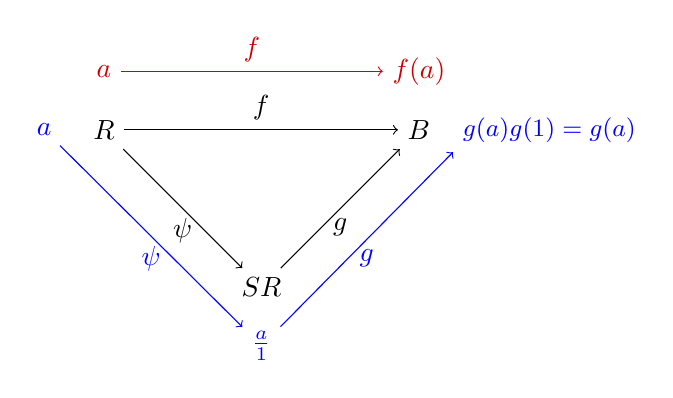
\begin{tikzpicture}
			\node (R) at (0,0) {$R$};
			\node (SR) at (2,-2) {$\inv{S}R$};
			\node (B) at (4, 0) {$B$};

			\draw[->] (R) -- node[midway, below] {$\psi$} (SR);
			\draw[->] (SR) -- node[midway, below] {$g$} (B);
			\draw[->] (R) -- node[midway, above] {$f$} (B);

			\node[blue, xshift = -0.5cm] (A) at (R.west) {$a$};
			\node[blue, xshift = 0.7cm, anchor = west] (AB) at (B.west) {\small $g(a)·\inv{g(1)} = g(a)$};
			\node[blue, yshift=-0.5cm] (A1) at (SR.south) {$\frac{a}{1}$};

			\draw[->, blue] (A) -- node[midway, below] {$\psi$} (A1);
			\draw[->, blue] (A1) -- node[midway, below] {$g$} (AB.south west);

			\node[red!80!black, yshift = 0.5cm] (FA) at (R.north) {$a$};
			\node[red!80!black, yshift = 0.5cm] (FB) at (B.north) {$f(a)$};

			\draw[->, red!80!black] (FA) -- node[midway, above] {$f$} (FB);
			\end{tikzpicture}
		\end{center}

		Por tanto, como el diagrama conmuta $g(a)=f(a)$, lo que nos deja fijo el comportamiento de $g$ en los elementos de la forma $\frac{a}{1}$ con $a ∈ R$. Nos falta saber qué ocurre con los que no son de esa forma, y saber si ahí también tenemos una única posibilidad de tomar $g$.

		Para eso, sólo tenemos que ver qué ocurre a los elementos de la forma $\frac{1}{s}$. Operando: \[ g(\frac{1}{s})=g(1)g(s^{-1})=g(s^{-1})=g(s)^{-1}=f(s)^{-1} \], ya que por hipótesis $f(s)$ con $s ∈ S$ son elementos invertibles. Por lo tanto, $g$ es única y depende solamente de la elección de la $f$ de partida.

		\proofpart{Existencia}

		Ahora vamos a probar que existe esa $g$. Si $g$ existiese tendríamos $g\left( \frac{r}{s}\right)=f(r)f(s)^{-1}$. Tenemos que ver que $g$ está bien definida (que dos elementos iguales no tengan imágenes distintas), es decir, que la expresión anterior no dependa del representante escogido.

		Supongamos que $\frac{r}{s} \equiv \frac{r'}{s'}$, hay que ver que $g\left(\frac{r}{s}\right)=g\left(\frac{r'}{s'}\right)$. Es decir, que $f(r)f(s)^{-1}=f(r')f(s')^{-1}$.

		Como  $\frac{r}{s} \equiv \frac{r'}{s'}$, entonces existe $s'' \in S$ tal que $s''(rs'-sr')=0$ en $R$. Aplicando f nos queda:
		$$f(s''(rs'-sr'))=f(s'')\left( f(r)f(s')-f(s)f(r') \right)=0$$

		Por hipótesis $f(s'')$ es invertible, por tanto, es una unidad en $B$, entonces no es un divisor de 0 y por tanto:
		$$f(r)f(s')-f(s)f(r')=0 \implies f(r)f(s')=f(s)f(r')$$

		Y multiplicando por la inversa de $f(s')$ y de $f(s)$, nos queda $f(r)f(s)^{-1}=f(r')f(s')^{-1}$.
	\end{proof}

	\begin{example}
		Sea $\rac[x]$, cogemos como parte multiplicativa $S=\{x^n\}$.

		Los elementos de $S^{-1}\rac[x]$ serán de la forma $\frac{p(x)}{x^m}$.

		\notacion $S^{-1}\rac[x]=\rac[x]_{\{x\}}$

		Defino el siguiente diagrama:

		\begin{center}
		\begin{tikzpicture}
		\matrix (m) [matrix of math nodes,row sep=4em,column sep=2em,minimum width=2em]
		{
			\rac[x] &  & \quot{\rac[x,y]}{\gen{xy-1}} \\
			& S^{-1}\rac[x]=\rac[x]_{\{x\}}  &  \\};
		\path[-stealth]
		(m-1-1) edge node [above] {$h$} (m-1-3)
		(m-1-1) edge node [below] {$\psi$} (m-2-2)
		(m-2-2) edge node [right] {$g$} (m-1-3);
		\end{tikzpicture}
		\end{center}

		Vemos que $\cls{x}\cls{y}=\cls{1} \implies x^{-1}=y \implies (x^m)^{-1}=y^m$. Con esto hemos visto que $h(s)$ es invertible $\forall s \in S$.

		La propiedad universal me dice que tengo un único homomorfismo $g: \rac[x]_{\{x\}}\longmapsto \quot{\rac[x,y]}{\gen{xy-1}}$

	\end{example}

	\begin{theorem} \label{thm:PropsLocalizacion}
		Sea $S \subset R$ una parte multiplicativa. El homomorfismo de paso al localizado $\psi:R \longmapsto S^{-1}R$ tiene las siguientes propiedades:
		\begin{enumerate}
			\item Si $s\in S$, $\psi(s)$ es invertible en $S^{-1}R$.
			\item $\psi(a)=0 \Leftrightarrow \exists s \in S$ tal que $s\cdot a=0$.
			\item Cada elemento de $S^{-1}R$ es de la forma $\psi(r)\psi(s)^{-1}$
		\end{enumerate}

		Estas propiedades determinan completamente a $S^{-1}R$ de tal modo que si $f:R \longmapsto B$ es un homomorfismo de anillos tal que se cumplen $1), 2), 3)$ (cambiando $S^{-1}R$ por $B$) entonces $S^{-1}R \simeq B$.
	\end{theorem}

	\begin{proof}
		\begin{tikzpicture}
		\matrix (m) [matrix of math nodes,row sep=4em,column sep=2em,minimum width=2em]
		{
			R &  &  B\\
			& S^{-1}R &  \\};
		\path[-stealth]
		(m-1-1) edge node [above] {$f$} (m-1-3)
		(m-1-1) edge node [below] {$\psi$} (m-2-2)
		(m-2-2) edge node [right] {$\exists g \text{ que conmuta el diagrama por la propiedad universal}$} (m-1-3);
		\end{tikzpicture}

		Veamos que ese $g$ es un isomorfismo:
		\begin{itemize}
			\item \textbf{g es sobreyectiva:} Si, por $3)$, todo elemento $a \in B$ es de la forma $f(r)f(s)^{-1}$. Tenemos que ver que para todo elemento de $B$ hay una preimagen en $S^{-1}R$ Basta observar que $g\left( \frac{r}{s} \right) f(r)f(s)^{-1}$.
			\item \textbf{g es inyectiva:} Si porque:
			$$\ker(g) = \{ \frac{r}{s}: g(r)g(s)^{-1}=0_B \} = \{ \frac{r}{s}: f(r)f(s)^{-1}=0_B \} = $$

			Y como $f(s)^{-1}$ es invertible, no es divisor de 0 y por tanto:

			$$ = \{ \frac{r}{s}: f(r)=0_B \} \implies r \in \ker(f) \implies r \in \ker(\psi)\textcolor{red}{???}$$
		\end{itemize}
	\end{proof}

\section{Ideales y localización}

\nota Esto es elemental, pero yo a veces lo dudaba. Sea cualquier función $f: A \longmapsto B$:
\begin{itemize}
	\item Sea un conjunto $M \subset B$, entonces $f(f^{-1}(M)) \subset B$.

	Intuitivamente, al hacer $f^{-1}(M)$ te quedas con los $x \in A$ tal que $f(x) \in M$, pero no todos los $m \in M$ tienen porque tener una preimagen $x \in A$..., por tanto es ahi donde empequeñece el conjunto. Si $f$ es sobreyectiva entonces $f(f^{-1}(M))= B$.
	\item Sea un conjunto $N \subset A$, entonces $f^{-1}(f(N)) \supset A$.

	Intuitivamente, al hacer $f(N)$ te quedas con los $y \in B$ tal que $f(x)=y$, con $x\in N$, pero puede que haya valores de $y$ que sean la imagen de dos valores distintos de $x$, y que alguno de ellos no pertenezca a $N$, es al hacer la preimagen de esos $y$ cuando podemos agrandar el conjunto. Si $f$ es inyectiva entonces $f^{-1}(f(N)) =  A$.
\end{itemize}

Vamos con lo importante, enunciaremos y demostraremos 4 proposiciones sobre ideales y localización. A lo largo de esta sección, consideraremos $\appl{\psi}{R}{S^{-1}R}$ nuestra aplicación de paso al localizado.

En general, si cogemos un ideal $J \subset S^{-1}R$, entonces $\psi^{-1}(J)$ es ideal en $R$. Pero si volvemos a tomar la imagen por ψ no tiene por qué ser un ideal. En secciones anteriores habríamos que podemos considerar el ideal extendido que sí está contenido en $J$: $\psi(\psi^{-1}(J))^e \subset J$. En el caso particular del paso al localizado, tendremos una igualdad.

\begin{prop}
	Sea $\psi:R \longmapsto S^{-1}R$ el homomorfismo de paso al localizado, y sea el ideal $J \subset S^{-1}R$.  Entonces $\psi(\psi^{-1}(J))^e = J$.
\end{prop}

\begin{proof}
	Ya tenemos $\psi(\psi^{-1}(J))^e \subset J$. Por tanto probamos $\psi(\psi^{-1}(J))^e \supset J$:

	Consideramos un elemento $\frac{b}{s} \in J$. Por ser $J$ ideal, tenemos que $\frac{b}{s} \frac{s}{1} = \frac{b}{1} ∈ J$, y su imagen inversa será $b ∈ \inv{ψ}(J)$.

	Ahora simplemente hacemos el camino de vuelta: $ψ(b) = \frac{b}{1} ∈ ψ(\inv{ψ}(J)) ⊂ \psi(\psi^{-1}(J))^e$. Como este último es un ideal, multiplicamos de nuevo $\frac{b}{1}$ por $\frac{1}{s}$ para tener por absorción que $\frac{b}{s} ∈ \psi(\psi^{-1}(J))^e$.
\end{proof}


\obs Todo ideal de $S^{-1}R$ es el extendido de algún ideal de $R$.

Si partimos de un ideal en $R$, también podemos tener un resultado para $\psi^{-1}(\psi(I)^e) $ que contendrá a $I$ (y quizás sea igual a él). Ahora bien, no será tan fácil como el anterior. Vamos a ver primero algunos ejemplos.

\begin{example}
	\begin{itemize}
		\item Sea $\psi: \ent \longmapsto \rac$. $\rac$ es localizado de $\ent$, haciendo invertible $S=\rac \setminus\gen{0}$. Nos queda $\rac=S^{-1}\ent$.

		Si cojo $I=2\ent \implies \psi(I)^e=\rac \implies \psi^{-1}(\psi(I)^e)= \ent$

		\item Sea $S=\{ 2^n \}$, $\psi: \ent \longmapsto \S^{-1}\ent$

		Sea $I=6\ent\implies 6\frac{1}{2}=3 \in \psi(I)^e$... ejemplo sin terminar...
	\end{itemize}
\end{example}

\begin{prop}
	$$\psi^{-1}(\psi(I)^e)=\bigcup_{s\in S}(I:S)$$

	Con $(I:S)=\{ r \in R: r\cdot S \in I \}$.
\end{prop}

\begin{proof}
	\begin{itemize}
		\item $\supset)$ Sea $r \in \bigcup_{s\in S}(I:S) \implies \exists s' \in S$ tal que $r \in (I:s')\implies r\cdot s' \in I \implies \frac{r \cdot s'}{1} \in \psi(I) \textcolor{red}{\implies} \frac{r}{1} \in \psi(I)^e \implies r \in \psi^{-1}(\psi(I)^e)$
		\item $\subset$ Sea $r \in \psi^{-1}(\psi(I)^e)\implies \frac{r}{1}\in \psi(I)^e \implies \frac{r}{1}=\frac{r_1}{s_1}a_1+...+\frac{r_t}{s_t}a_t$ con $a_1,...,a_t \in I \implies s''\frac{r}{a}\in I$ con $s''=s_1...s_t \implies r \in (I:s'')$
	\end{itemize}
\end{proof}

\begin{prop} $\psi^{-1}(\psi(I)^e)=R \Leftrightarrow I \cap S \neq \emptyset$.
\end{prop}

\begin{prop}
	Sea $\pideal \subset R$ un ideal primo, entonces:
	\begin{itemize}
		\item Si $\pideal \cap S \neq \emptyset \implies \psi(\pideal)^e=S^{-1}R$.
		\item Si $\pideal \cap S = \emptyset \implies \psi(\pideal)^e$ es un ideal primo en $S^{-1}R$.
	\end{itemize}
\end{prop}

\begin{proof}
	Vamos a probar que $\psi(\pideal)^e$ es primo.

	Tenemos que $\psi(\pideal)^e\neq \gen{1}$ porque $\pideal \cap S= \emptyset$

	Sean $\frac{r}{s},\frac{r'}{s'} \in S^{-1}R$ tal que $\frac{r}{s}\cdot\frac{r'}{s'} \in \psi(\pideal)^e$.

	Entonces $\frac{r}{s}$ o $\frac{r'}{s'} \in \psi(\pideal)^e \implies \frac{r}{s}\cdot\frac{r'}{s'}=\frac{r_1}{s_1}a_1+...+\frac{r_t}{s_t}a_t$ con $a_1,...,a_t \in \pideal$ y $s_1,...,s_t \in S$.

	Sea $s''=s\cdot s' \cdot s_1 \cdot...\cdot s_t \in S$. Definimos: $\cls{s}=\frac{s''}{s\cdot s'} \in S \subset R$. Entonces:
	$$ \underbrace{\frac{s''}{s\cdot s'}}_{\in S \subset R}\cdot r \cdot r'=\underbrace{s''\frac{r_1}{s_1}a_1+...+s''\frac{r_t}{s_t}a_t}_{\text{comb lineal sobre R de elementos de }\pideal} $$

	Por tanto $(\cls{s})\cdot(r \cdot r') \in \pideal$ que es primo $\implies \underbrace{\cls{s}\in p}_{\textbf{No porque}\pideal \cap S = \emptyset}$ o $r\cdot r' \in \pideal \implies r \cdot r' \in \pideal \implies r$ o $r' \in \pideal$.

	Si $r \in \pideal \implies \frac{r}{1} \in \psi(\pideal)$ y $\frac{r}{s} \in \psi(\pideal)^e$. Si no, de igual modo se prueba que entonces $\frac{r'}{s'}\in \psi(\pideal)^e$.
\end{proof}

Las conclusiones de estas tres proposiciones son \textbf{IMPORTANTES}:
\begin{enumerate}
	\item Todo ideal de $S^{-1}R$ es el extendido de algún ideal de $R$.
	\item Hay una correspondencia biyectiva entre ideales primos $p \subset R$, $p \cap S = \emptyset$ y los ideales primos de $S^{-1}R$.
\end{enumerate}

\notacion
\begin{itemize}
	\item Sea $S \subset R$, $S=\{ a^n \}, a \in R$. Entonces $S^{-1}R=R_a=R_{\{a\}}$. A esto se le llama ``R localizado en a'' o \concept{Localización\IS en un elemento}.
	\item Sea $S=R \setminus \pideal$ con $\pideal \subset R$ ideal primo en $R$. Entonces $S^{-1}R=R_\pideal$. A esto se le llama ``R localizado en el ideal primo $\pideal$'' o \concept{Localización\IS en un ideal primo}, y además $R_\pideal$ es un anillo local.
\end{itemize}


Sea $R=\ent$, no confundir: $\ent_{\{3\}}$, con $\ent_{\gen{3}}$ con $\ent_3$, son todos distintos. Observar que con $R=\ent$ es diferente $R_a$ y $R_{\{a\}}$.
\begin{itemize}
	\item $\ent_{\{3\}}$ es un subanillo de los racionales en el que sólo nos quedamos con aquellos números racionales que admiten una escritura cuyo denominador es una potencia de 3.
	\item $\ent_{\gen{3}}$ es un subanillo de los racionales en el que sólo nos quedamos con aquellos números racionales que admiten una escritura cuyo denominador no es un múltiplo de 3.
	\item $\ent_3=\{ \cls{0},\cls{1},\cls{2} \}$ que no tiene nada que ver con todo esto.
\end{itemize}

\section{Anillos noetherianos}
\begin{defn}[Anillo\IS noetheriano] \label{def:AnilloNoetheriano}
	Se dice que $R$ es un anillo noetheriano si todo ideal $I \subset R$ es finitamente generado (como $R$-módulo). (ver \nref{def:rmodulo_fg})

	%Es decir, que para todo ideal en R  puedo encontrar un número finito de elementos dentro del ideal, de modo tal que cualquier otro elemento que viva en el ideal se puede escribir como combinación lineal de ellos.
\end{defn}

\begin{example}
	\begin{itemize}
	\item $\ent$ es noetheriano, porque es dominio de ideales principales, es decir, todos sus ideales son principales (ver \nlref{def:ideal_principal}).
	\item $K$ cuerpo es noetheriano, porque en un cuerpo solo hay dos ideales, $\{0\}$ y $K$, ambos finitamente generados.
	\item $K[x]$ es noetheriano, porque es dominio de ideales principales.
	\item $K[x_1,...,x_n]$, $\rac[x,y]$ y $\ent[x]$ son noetherianos, pero hay que demostrarlo.
	\item $K[x_1,...,x_n,...]$, con número infinito de variables no es noetheriano.

	Cogemos $I \subset K$, $I= \{ p(\cls{x}): \text{término constante igual a 0} \}$.

	\notacion $\cls{x}=\{x_1,x_2,...,x_n,...\}$
	\nota En $I$ no existe el polinomio $p(\cls{x})=x_1+x_2+...+x_n+...$ ya que no se pueden sumar un número infinito de sumandos. Las combinaciones lineales finitas sí están.

	Entonces tenemos que $I$ es un ideal (cumple las tres condiciones de los ideales), y que $p(\cls{x})=x_i \in I$ $ \forall i$. Pero $I$ no es finitamente generado.
	\begin{proof}
		Supongamos que $\exists p_1,...,p_s \in K[x_1,...,x_n,...]$ tal que $I=\gen{p_1,...,p_s}$, tal que $p_1,...,p_s$ solo dependen de un número finito de variables.

		Supongamos sin pérdida de generalidad que sólo dependen de $x_1,...,x_n$.

		Entonces es imposible escribir $x_{n+1}$ como combinación de los $p_i$. $x_{n+1}\neq q_1p_1+...+q_sp_s$, como mucho obtenemos productos $x_ix_{n+1}$, pero nunca $x_{n+1}$ solo.
	\end{proof}
	\end{itemize}
\end{example}

\begin{prop}\label{prop:caracterizacion_noetheriano}
	Son equivalentes:
	\begin{enumerate}
		\item $R$ es noetheriano.
		\item Toda cadena creciente de ideales en $R$, $\{I_i\}_{i \in \nat}$ estabiliza para un $n$ suficientemente grande: $I_1 \subseteq I_2 \subseteq ... \subseteq I_n = I_{n+1}$.
		\item Todo conjunto no vacío de ideales en $R$ tiene un elemento maximal (No tiene por qué ser un ideal maximal).
	\end{enumerate}
\end{prop}

\begin{proof}

		\proofpart{$1) \implies 2)$}

		Sea $R$ un anillo noetheriano y sea $\{I_i\}_{i \in \nat}$ una cadena creciente de ideales en $R$. Queremos probar que la cadena estabiliza para algún $N$ suficientemente grande.

		Sea $J= \bigcup_{i \in \nat} I_i$. Entonces $J$  es un ideal en $R$. En general la union de ideales no tiene porque ser un ideal, pero en el caso de ser una cadena creciente sí lo es (mirar demostración del teorema \ref{thm:IdealContenidoMaximal}). Como $R$ es noetheriano, $J$ es finitamente generado, por tanto existen $a_1,...,a_s \in J$ tal que $J=\gen{a_1,...,a_s}$.

		Además tenemos que $I_1 \subseteq I_2 \subseteq ... \subseteq I_N \subseteq ...$, por tanto, $\exists k$ tal que  $a_1,...,a_s \in I_k = J = \gen{a_1,...,a_s}$

		\proofpart{$2) \implies 3)$}

		Sea $\Sigma$ un conjunto no vacío de ideales en $R$, queremos probar que tiene un elemento maximal.

		Supongamos que en $\Sigma$ hay una cadena creciente de ideales $\{I_i\}$. Por la hipótesis en $2)$, la cadena estabiliza, luego tiene un elemento maximal.

		Si esa cadena no existe, se construye. Tenemos un conjunto de ideales $\set{I_i}$, así que construimos la cadena $I_1 ⊆ I_1 ∪ I_2 ⊆ I_1 ∪ I_2 ∪ I_3 ⊆ \dotsb$ y aplicamos lo de antes\footnoteby{Guille}{No tengo claro qué hacer si el conjunto de ideales es no numerable. Ahora bien, parece que ese no es un caso que estemos considerando en ningún momento.}.

		\proofpart{$3) \implies 1)$}

		Sabemos que todo conjunto no vacío de ideales en $R$ tiene un elemento maximal, y queremos probar que $R$ es noetheriano.

		Sea $I \subset R$, supongamos que $I\neq \{0\}$ y que $I$ no es finitamente generado.
		\begin{itemize}
			\item Sea $a_1 \in I, a_1 \neq 0$.
			\item Sea $a_2 \in I\setminus \gen{a_1}$. Puedo encontrar ese $a_2$ porque si no lo encontrara querría decir que $I$ sería finitamente generado.
			\item Sea $a_3 \in I\setminus \gen{a_1,a_2}$.
			\item Sea $a_n \in I\setminus \gen{a_1,...,a_n}$.
		\end{itemize}
		Considero $\gen{a_1}\subsetneq \gen{a1,a2} \subsetneq \gen{a_1,a_2,a_3} \subsetneq...$. Esta cadena creciente de ideales nunca estabiliza. Lo cual es contradictorio porque entonces podría haber definido $\Sigma=\{ \gen{a_1}, \gen{a_1},\gen{a_1,a_2},...,\gen{a_1,a_2,...,a_n},.... \} \neq \emptyset$ y no tiene elemento maximal.
\end{proof}

\begin{theorem}[Teorema\IS de la base de Hilbert]\label{thm:tma_base_hilbert}
	Sea $R$ un anillo noetheriano. Entonces $R[x]$ es un anillo noetheriano.
\end{theorem}

\begin{proof}
	Sea $I \subset R[x]$, queremos probar que $I$ es finitamente generado.
	\nota El coeficiente director de un polinomio es el coeficiente que acompaña al término de mayor grado.
	\nota El grado es un numero $a \in \nat$, y los $\nat$ son ordenables, por tanto, si hablamos de grado mínimo, que no nos extrañe, es lo que todos pensamos: el grado menor.

	Vamos a suponer que $I$ no es finitamente generado, podemos suponer que $I\neq \{0\}$, así:
	\begin{itemize}
		\item Sea $f_1(x) \in I$ con grado mínimo, sea $a_1$ el coeficiente director de $f_1(x)$.
		\item Sea $f_2(x) \in I\setminus \gen{f_1(x)}$ con grado mínimo, puedo cogerlo ya que hemos supuesto que $I$ no es finitamente generado, sea $a_2$ el coeficiente director de $f_2(x)$.
		\item Sea $f_{k+1}(x) \in I\setminus \gen{f_1(x),...,f_k(x)}$ con grado mínimo, sea $a_{k+1}$ el coeficiente director de $f_k(x)$.
	\end{itemize}

	Entonces, con los coeficientes directores puedo montar la siguiente cadena: $\gen{a_1} \subseteq \gen{a_1,a_2} \subseteq ... \subseteq \gen{a_1,...,a_k,a_{k+1}}$, que es una cadena creciente de ideales de $R$, además sabemos por hipótesis que $R$ es noetheriano, por tanto esa cadena se debe estabilizar.

	Pero hemos supuesto que $I$ no es finitamente generado, y afirmamos que si eso ocurre, la cadena anterior no puede estabilizar, vamos a probar eso:

	Supongamos que estabiliza $\implies$ para algún $k$ se cumple que $\gen{a_1,...,a_k}=\gen{a_1,...,a_k,a_{k+1}} \implies \exists b_1,...,b_k \in R$ tal que: $a_{k+1}=b_1a_1+...+b_ka_k$. Donde $a_{k+1}$ es el coeficiente director de $f_{k+1}(x)$. Defino:

	\textcolor{red}{Revisar el final de esta demostracion}

	$$ g=f_{k+1}(x)-\sum_{i=1}^{k}b_ix^{\deg(f_{k+1}(x))-\deg(f_i(x))} f_i(x) \in I\setminus \gen{f_1,...,f_k} $$

	%Como las $f_i$ tiene grado igual o mayor, estoy haciendo es obtener justamente el a_{k+1} con signo negativo.

	Tenemos que $\deg(g) < \deg(f_{k+1}(x))$. Lo cual es contradictorio porque $g \in I \setminus \gen{f_1,...,f_k}$ y tiene grado < $\deg(f_{k+1})$.

\end{proof}

\begin{example}
	\begin{itemize}
	\item $\ent[x_1,...,x_n]$ es noetheriano. No hay más que coger $\ent$, que sabemos que es noetheriano, y 'aplicar' el teorema anterior n veces.
	\item $\K[x_1,...,x_n]$ es noetheriano por el mismo motivo.
	\item Si $R$ es noetheriano $\implies$ $R[x_1,...,x_n]$ es noetheriano.
	\end{itemize}
\end{example}

\subsection{Anillos noetherianos y paso al cociente}

\begin{prop} \label{prop:NoetherianoCociente}
	Sea $R$ un anillo noetheriano y sea $I \subset R$ un ideal $\implies$ $\quot{R}{I}$ también es noetheriano.
\end{prop}
\begin{proof}
	Sea $\pi: R \longmapsto \quot{R}{I}$, tenemos que probar que $J \subset \quot{R}{I}$ es finitamente generado.

	Cogemos $L \subset R$ ideal de $R$ tal que $I \subset L$ y tal que $\pi(L)=J$ ($L$ es posible de encontrar, ver \ref{relacionRconRI}, relación entre los ideales de $R$ y $\quot{R}{I}$, apartado 2). Como $R$ es noetheriano, $L$ es finitamente generado, es decir, $\exists a_1,...,a_s \in L$ tal que $L=\gen{a_1,...,a_s} \implies J=\gen{\pi(a_1),...,\pi(a_s)}$.

	También se puede probar utilizando la segunda caracterización de los anillos noetherianos (ver proposición \ref{prop:caracterizacion_noetheriano}). Cualquier cadena creciente de ideales en $R$ estabiliza, si me fijo en una cadena creciente de ideales en $\quot{R}{I}$, viene de una cadena creciente de ideales en $R$, por la correspondencia biyectiva.
\end{proof}

Una consecuencia de lo anterior es:

\obs Sea $R$ un anillo noetheriano y sea $T$ una $R$-álgebra de tipo finito (ver definición de $R$-álgebra finitamente generada: \ref{def:ralgebra_fg}). Entonces $T=R[b_1,...,b_n]$ para ciertos $b_1,...,b_n \in T$. De hecho $T=R[b_1,...,b_n]$ es también noetheriano.

\begin{proof}
	Sea $R$ un anillo noetheriano, le añadimos n variables (sigue siendo noetheriano por el teorema de Hilbert \ref{thm:tma_base_hilbert}) y definimos el siguiente homomorfismo de $R$-álgebras:

	\begin{align*}
		\psi: R[x_1,...,x_n] & \longmapsto  T=R[b_1,...,b_n]\\
		r \in R & \longmapsto r \\
		x_i & \longmapsto b_i \\
	\end{align*}

	Entonces $\psi$ es un homomorfismo de $R$-álgebras y es sobreyectivo por cómo lo hemos construido. Ahora aplicamos el primer teorema de isomorfía:
	$$ \quot{R[x_1,...,x_n]}{\ker(\psi)} \simeq \img(\psi)=T=R[b_1,...,b_n]$$

	Por tanto tenemos:
	 $$\quot{\text{anillo noetheriano}}{\text{ideal}}$$

	Y como hemos visto antes, eso es noetheriano. Por tanto: $T=R[b_1,...,b_n]$ es noetheriano.
\end{proof}

\begin{example}
	\begin{itemize}
		\item $\rac[\sqrt{2},x, \pi]$ es una $\rac$-álgebra.
		\item $\real$ es una $\rac$-álgebra pero no de tipo finito.
	\end{itemize}
\end{example}

\subsection{Anillos noetherianos y localización}

\begin{prop} \label{prop:NoetherianoLocalizacion}
	Sea R un anillo noetheriano y sea $S\subset R$ una parte multiplicativa. Construimos como otras veces el siguiente homomorfismo:
	$$\psi: R \longmapsto S^{-1}R$$

	Entonces $S^{-1}R$ es noetheriano.
\end{prop}
\begin{proof}
	Para ello tenemos que probar que sea $J \subset S^{-1}R$ un ideal, este es finitamente generado.

	Lo cual es cierto ya que $J$ es el extendido de algún ideal de $R$ y hemos probado que $\psi(\psi^{-1}(J))^e=J$. Por tanto $J$ es el extendido de $\psi^{-1}(J)\subset R \implies J$ es finitamente generado. \textcolor{red}{Revisar cuando repase lo que dimos esos días...} %min 19
\end{proof}


